% =====================================================================================
% sections/evaluation.tex: Evaluation (IEEE S&P 2027 submission, condensed per CUT_PLAN.md).
% Sources: wt_sp2027/report (tables llm, cnn, hardware; Secs. 3.6, 4), SP2027_PLAN.md, and
%   docs/improvements/{A1,A2,A3,B2_B3,B5,C2,D4_D5,F1}.md; numbers unchanged from the draft. Derived
%   by arithmetic only: V1 ratios, the bandwidth crossover (0.16-0.26 Gb/s, MB = 10^6 bytes),
%   factors against published systems. Removed material: sections/ext_evaluation.tex.
% Labels defined: sec:results, sec:eval-setup, sec:eval-cost, sec:eval-v1, sec:eval-reexec,
%   sec:eval-compare, tab:eval-llm, tab:eval-v1, tab:eval-reexec, tab:eval-compare.
% Labels used: sec:break, sec:defence, sec:v1, sec:quality (quality.tex), tab:sok; cite fullversion.
% Second trimming pass (2026-10-10): -110 words; dropped only facts stated elsewhere (hash/field
%   choices: defence.tex; F_{p^8}: v1.tex; image-model list: attack.tex Sec. sec:break; cell values
%   repeated from the tables); the GKR time per leaf moved to ext_evaluation.tex (app:eval-gkr-leaf).
% H5 pass (2026-10-11, REVIEW2.md): P3 (the two LeNet-5 rows of tab:eval-compare moved to
%   ext_evaluation.tex), C7 (per-row factors of the comparison paragraph removed), N3 (footnote a of
%   tab:options labels the re-execution rows: GPU before the int8 forward pass, F1 Sec. 3 and A2;
%   CPU weight products as fp32 GEMMs over 1,024-term chunks, A2 Sec. 3), N4 (tab:eval-v1 caption,
%   "Time" and "Bandwidth crossover" label the earlier v0 verifier; V-LONG-a todo), N8 ("0.12 against
%   0.14 s" deleted: no source in docs/improvements; B5 Sec. 6 has 0.278 against 0.153 s for an
%   earlier kernel), N9 (one source for real weights: 1.78-1.85x, C2_v1_proof_size.md Sec. 8),
%   smaller note (tab:options caption names the protocol mode).
% =====================================================================================

\providecommand{\Kpre}{\mathsf{K}_{\mathrm{pre}}}
\providecommand{\sC}{\mathsf{C}}
\providecommand{\sK}{\mathsf{K}}
\providecommand{\para}[1]{\par\noindent\textbf{#1}\quad}
\providecommand{\todo}[1]{\textbf{[TODO: #1]}}

\section{Evaluation}
\label{sec:results}

We measure the cost of the defence (Section~\ref{sec:eval-cost}), V1 against v0
(Section~\ref{sec:eval-v1}), verification against re-execution (Section~\ref{sec:eval-reexec}),
published systems (Section~\ref{sec:eval-compare}) and the quality of the certified model
(Section~\ref{sec:quality}).

% -------------------------------------------------------------------------------------
\subsection{Setup}
\label{sec:eval-setup}

\para{Implementation.} The protocol is written in Python and PyTorch, with Triton kernels for the
GPU claim decoder and the fused exact attention, and C++/OpenMP kernels for CPU
verifiers. We use $\lambda = 128$ unless stated otherwise; v0 and V1 are the protocols of
Sections~\ref{sec:defence} and~\ref{sec:v1}.

\para{Platform.} The final tables will come from one platform: an NVIDIA L40S (48\,GB) as prover
and GPU verifier and one CPU for the CPU verifier and re-execution, with full models, no
extrapolation, and medians with their spread \todo{L40S}. The numbers shown come from earlier runs:
the \emph{base} implementation on the L40S with 8 threads of an AMD EPYC 9334, the later
improvements and V1 on an RTX~2080~Ti (11\,GB) with 8 threads of an Intel Xeon Silver 4114, each
against the previous code (or v0) on the same queries with identical claims, proofs and verdicts.
Times are medians after a warm-up.

\para{Models.} The image models are the six of Section~\ref{sec:break}. The language models are
GPT-2, OPT-125M/1.3B/6.7B, Llama-2-7B/13B and Qwen3-4B. Costs use random int8 weights, since they
depend only on the shapes, except for the compressed size of the claims. Real weights confirm
this: on the smoothed OPT-1.3B (both modes, 64 and 2{,}048 tokens) the prover's and the CPU
verifier's times are within \RealProveWithin{}\% and \RealVerifyWithin{}\% of random weights', and v0's proof is \RealProofSmaller{}\% smaller;
the full real OPT-6.7B and OpenLLaMA-7B (Llama-2-7B's shapes) in $\Kpre$ at 2{,}048 tokens are
accepted, and every tamper rejected~\cite{fullversion}. A model too large for the 2080~Ti is measured
as $b$ of its $L$ blocks ($b/L$), the last one pruned.

\para{Attacks and soundness tests.} Section~\ref{sec:break} reports the attack measurements. Our
base verifier accepted all \FinalNHonest{} honest queries and rejected all \FinalNAttacks{} attacks (one changed
value or neuron, perturbed weights, substitute models, forgeries that pass all checks but one):
Freivalds' check rejected \FinalNFreivalds{}, the column check \FinalNColumnsCode{}, the Merkle check \FinalNColumnsMerkle{} and the range check \FinalNRange{}\TodoCounts{}.

% -------------------------------------------------------------------------------------
\subsection{Cost of the Defence}
\label{sec:eval-cost}

\begin{table*}[t]
  \caption{Cost of proving the next-token logits of one prompt (interactive, $\lambda{=}128$, random
  int8 weights). Base: before the improvements, on an NVIDIA L40S (prover, GPU verifier) and
  8 threads of an AMD EPYC 9334 (CPU verifier). New: all improvements, on the L40S. Proof bytes do
  not change (--: not measured). New CPU verifier: \todo{L40S/EPYC}}
  \label{tab:eval-llm}
  \centering\footnotesize
  \setlength{\tabcolsep}{3.5pt}
  \begin{tabular}{@{}lrrrrrrrrr@{}}
    \toprule
    & & \multicolumn{6}{c}{committed weights ($\sC$)} & \multicolumn{2}{c}{$\Kpre$} \\
    \cmidrule(lr){3-8}\cmidrule(l){9-10}
    & & \multicolumn{2}{c}{prove} & CPU verify & \multicolumn{2}{c}{GPU verify} & & CPU verify & \\
    \cmidrule(lr){3-4}\cmidrule(lr){6-7}
    Model & Params & base & new & base & base & new & proof & base & proof \\
    \midrule
    \pvitable{tab_eval_llm}
    \bottomrule
  \end{tabular}
\end{table*}

\para{Base costs.} With committed weights, the image models are proved in \CnnProveRange{}\,ms and
verified in \CnnVerifyRange{}\,ms, with proofs \CnnProofRatio{}$\times$ smaller than their int8 weights.
Llama-2-7B's 64-token proof is about \ProofRatioLlamaShort{}$\times$ smaller than its int8 weights
(Table~\ref{tab:eval-llm}). At 2{,}048 tokens the proof and the CPU verifier's time grow
(OPT-6.7B: \ProofOptLLong{}, \VerifyOptLLong{}), since the results of the weight operations grow with the prompt (\ClaimsShareLlama{}\%
of Llama-2-7B's \ProofLlamaLongCExact{} proof) and the verifier recomputes attention over all pairs of positions.
There the GPU verifier is \GpuVerifyFactor{}$\times$ faster than the CPU one \todo{F6 (F4): peak memory}.
On one RTX~2080~Ti, proving a 2{,}048-token OPT-1.3B prompt takes \ServeOptMKpre{}\,s in $\Kpre$ and \ServeOptMC{}\,s in
$\sC$: \ServeOptMKpreOverUOne{} and \ServeOptMCOverUOne{}$\times$ our exact integer forward pass without proofs, and \ServeOptMKpreOverUTwo{} and \ServeOptMCOverUTwo{}$\times$ an
fp16 one. Proving 64 prompts of 64 tokens together in $\Kpre$ takes \ServeBatchKpre{}\,s (\ServeBatchOverUOne{} and
\ServeBatchOverUTwo{}$\times$)\TodoServing{}.

\para{Improvements.} Our improvements change no byte that the parties exchange; the extended
version~\cite{fullversion} measures each against the previous code path. Exact int8 GEMMs for the
column opening, which took 62\% of Llama-2-7B's base prover at 64 tokens, and the fold make the
prover \ImproveOpenRange{}$\times$ faster on Llama-2 blocks, and a GPU claim decoder with a fused exact
attention kernel makes the GPU verifier \ImproveGpuvRange{}$\times$ faster at 2{,}048 tokens.

% -------------------------------------------------------------------------------------
\subsection{V1 Against v0}
\label{sec:eval-v1}

\begin{table}[t]
  \caption{V1 against v0 on the same queries (Fiat--Shamir, random int8 weights; --: not timed).
  Times: RTX~2080~Ti prover, 8 threads of a Xeon Silver 4114, from a run with GKR instances of at
  most $2^{24}$ leaves, whose proofs are within 0.3\,MB of those shown ($2^{27}$ leaves); the v0
  verifier times predate the final CPU kernels of Section~\ref{sec:eval-reexec}}
  \label{tab:eval-v1}
  \centering\footnotesize
  \setlength{\tabcolsep}{2.3pt}
  \begin{tabular}{@{}llrrrrr@{}}
    \toprule
    & & \multicolumn{3}{c}{proof (MB)} & prover (s) & verifier (s) \\
    \cmidrule(lr){3-5}
    Build ($b/L$) & mode & v0 & V1 & ratio & v0 / V1 & v0 / V1 \\
    \midrule
    \pvitable{tab_eval_v1}
    \bottomrule
  \end{tabular}
\end{table}

\para{Proof size.} At 2{,}048 tokens, with random weights, V1's proof is \VOneRatioRandom{}$\times$ smaller
than v0's on every build with more than one block (Table~\ref{tab:eval-v1}). V1's own additions
stay below 1\,MB per proof. The gain is smaller where the parts that V1 leaves unchanged weigh
more: the single Llama-2-13B block in $\sC$ (\VOneRatioLargeC{}$\times$), whose opened columns are a larger
share, and GPT-2 at 64 tokens (\VOneRatioShort{}$\times$). With real weights our design estimate is
1.78--1.85$\times$ at 2{,}048 tokens, and the smoothed real OPT-125M measures 1.68$\times$ ($\sC$)
and 1.77$\times$ ($\Kpre$) at 512 tokens, and the real OPT-6.7B \VOneRatioRealOptLExact{}$\times$ ($\Kpre$) at 2{,}048
tokens.

\para{Time.} The prover pays for the GKR, about one leaf per sent value. At 2{,}048 tokens V1's
prover thus takes about 10$\times$ as long as v0's (OPT-125M in $\sC$: \VOneOptSProveVZero{} to \VOneOptSProveVOne{}\,s, \VOneOptSGkr{}\,s of
it the GKR). The CPU verifier takes \VOneVerifyRatioLong{}$\times$ v0's time at 2{,}048 tokens and
\VOneVerifyRatioMedium{}$\times$ at 512, mostly for the two exact products per value of its final check; these
ratios use the earlier v0 verifier. Against the final v0 kernels the gap is wider: for the full
Llama-2-7B in $\Kpre$ at 2{,}048 tokens (Fiat--Shamir, V1 extrapolated from 2--3 blocks), V1's
verifier, with native kernels for its final check, takes \VOneVerifyLlama{}\,s and v0's \VOneVZeroVerifyLlama{}\,s, \VOneVerifyRatioLlama{}$\times$\TodoVOneTimings{}.


% -------------------------------------------------------------------------------------
\subsection{Verification Against Re-Execution}
\label{sec:eval-reexec}

\begin{table}[t]
  \caption{A client's options for one Llama-2-7B prompt of $T$ tokens, from this
  section and the cited papers, on different hardware (--: none or not reported;
  ours interactive, the V1 row under Fiat--Shamir, against v0's final verifier;
  CPU: 8 threads of a Xeon Silver 4114, full models, ours in $\Kpre$ with the native kernels,
  re-execution the fastest exact one; ours in $\sC$: EPYC 9334; GPU:
  RTX~2080~Ti) \todo{F6: $\sC$ at 2{,}048}}
  \label{tab:options}
  \centering\footnotesize
  \setlength{\tabcolsep}{2.2pt}
  \begin{tabular}{@{}llrrrrl@{}}
    \toprule
    & & \multicolumn{2}{c}{bytes per query} & \multicolumn{2}{c}{client time} & \\
    \cmidrule(lr){3-4}\cmidrule(lr){5-6}
    Option$^f$ & Holds & $T{=}64$ & 2{,}048 & $T{=}64$ & 2{,}048 & Guarantee \\
    \midrule
    \pvitable{tab_options}
    \bottomrule
  \end{tabular}

  \smallskip
  \parbox{\columnwidth}{\footnotesize $^a$Exact. CPU: the faster of the integer forward pass (64
  tokens) and fp32 (2{,}048); a non-exact int8 engine takes \DynIntShort{}/\DynIntLong{}\,s. GPU: the integer forward
  pass on int8 tensor cores (extrapolated from 1--2 blocks); fp16 takes \GpuFloatShort{}/\GpuFloatLong{}\,s. $^b$An edit passes a one-token response with probability about
  99.4\% at a 5\% audit rate (Table~\ref{tab:sok}). $^c$Designated verifier. $^d$The claims divided by V1's
  measured \VOneRatioLlama{}$\times$ (random weights; \VOneRatioRealOptLExact{}$\times$ on the real OPT-6.7B); its verifier under
  Fiat--Shamir.
  $^e$Llama-3.1-8B (Llama-2-7B's layers and width), per audited token, as
  reported~\cite{commitllm2026}: retained trace state (Merkle paths not counted) and the routine
  10-layer check on an Apple M4. $^f$Provider's cost over unverified serving: GPU TEE below
  7\%~\cite{gpucc}, CommitLLM 12--14\%~\cite{commitllm2026}; ours \ServeLlamaKpreOverUTwo{}$\times$ ($\Kpre$) and
  \ServeLlamaCOverUTwo{}$\times$ ($\sC$) fp16 inference on one RTX~2080~Ti (Llama-2-7B, extrapolated from 1--2
  blocks).}
\end{table}

\begin{figure}[t]
  \centering
  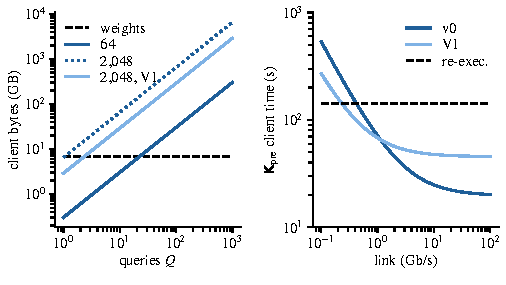
\includegraphics[width=\columnwidth]{figures/ev_breakeven.pdf}
  \caption{When a client of Llama-2-7B gains (random int8 weights, Fiat--Shamir). Left: the
  client's bytes for $Q$ mode-$\sC$ queries of 64 or 2{,}048 tokens, and with V1, against one
  download of the int8 weights (\WeightsLlamaGB{}\,GB). Right: a $\Kpre$ client's time for one 2{,}048-token
  query, transfer plus verification on 8 Xeon threads, against the fastest exact re-execution on the
  same threads (\CpuReexecLong{}\,s, \CpuReexecName{}), by link speed}
  \label{fig:breakeven}
\end{figure}

Table~\ref{tab:options} sets our verifier against exact re-execution, which only a client in $\sK$
or $\Kpre$ can run, and against the other options of a client.

\para{CPU.} With native exact kernels for every phase (an AVX-512 integer attention fused with its
requantisation, one-pass recomputed operations, field products and claim decoding), our $\Kpre$
verifier checks a 2{,}048-token query of the full Llama-2-7B in 18.5\,s on 8 threads of the Xeon
(\CpuVerifyLong{}\,s non-interactive), against \CpuReexecLong{}\,s for the fastest exact re-execution on the same threads
(\CpuReexecName{}; the exact integer forward pass takes \CpuReexecIntLong{}\,s): 5.0$\times$ (\CpuRatio{}$\times$) faster. At 64
tokens it takes 1.0\,s (\CpuVerifyShort{}\,s), against \CpuReexecShort{}\,s for the integer forward pass: 4.0$\times$
(\CpuRatioShort{}$\times$). The
CPU times of Table~\ref{tab:eval-llm} predate the kernels \todo{EPYC: the same cells}.

\para{Break-even.} A client that receives a proof of $B$ bytes over a link of $L$ bit/s and
verifies it in $t_v$ is faster than a re-execution taking $t_r$ when $L > 8B/(t_r - t_v)$.
Figure~\ref{fig:breakeven} plots this condition, and the client's bytes against one download of
the weights, for the cells above.

\para{GPU.} On a GPU, re-execution is faster.
With our verifier improvements, OPT-1.3B in $\Kpre$ extrapolates to about \OptMGpuVerify{}\,s on the 2080~Ti,
against \OptMGpuFloat{}\,s for its fp16 re-execution\TodoGpuOneGpu{}. We do not claim that
verification beats re-execution on a GPU; the GPU verifier suits an auditor or gateway that checks a
provider without holding the weights.

% -------------------------------------------------------------------------------------
\subsection{Comparison with Published Systems}
\label{sec:eval-compare}

\begin{table*}[t]
  \caption{Our costs against published systems on matched models, as reported on their own
  hardware. Ours: base implementation, v0 (bold where lower; in parentheses, ours lower
  $\downarrow$ or higher $\uparrow$ by the factor shown)}
  \label{tab:eval-compare}
  \centering\footnotesize
  \setlength{\tabcolsep}{2.5pt}
  \begin{tabular}{@{}llrrrrrr@{}}
    \toprule
    & & \multicolumn{2}{c}{prover} & \multicolumn{2}{c}{verifier} & \multicolumn{2}{c}{proof} \\
    \cmidrule(lr){3-4}\cmidrule(lr){5-6}\cmidrule(l){7-8}
    System & Model ($T$) & theirs & ours & theirs & ours & theirs & ours \\
    \midrule
    \pvitable{tab_eval_compare}
    \bottomrule
  \end{tabular}

  \smallskip
  \parbox{\textwidth}{\footnotesize Ours: NVIDIA L40S prover; verifier on 8 threads of an AMD
  EPYC 9334, or our GPU verifier in the 2{,}048-token rows, as zkLLM runs on a GPU; committed
  weights and Fiat--Shamir, except against zkLLM, which is interactive (so are ours there), and
  against Maverick. $^a$Verifier on one core. $^b$No prompt length stated (its shapes imply
  32 tokens). $^c$BaseFold configuration, proving every position. $^d$Maverick's client stores an
  encoded copy of the weights, so ours run in $\Kpre$, $\lambda{=}40$, one thread, without the
  compact encoding; Maverick draws a fresh challenge per query and proves on 64 CPU threads.}
\end{table*}

Table~\ref{tab:eval-compare} sets our costs against published
systems~\cite{zkcnn,zkml,zkgpt,deepprove,zktorch,maverick,zkllm} on matched models
(costs checked against the sources). Two caveats apply to every row. The hardware differs: our
prover runs on an L40S, while all the zkSNARKs except zkLLM ran on CPUs. The guarantees differ: the
zkSNARKs also prove the operations without weights, and many hide the weights; our verifier
recomputes those operations and our protocol is not zero-knowledge.
With these caveats, our prover is faster in every measured row, by \CompareProverMin{}$\times$ to about
\CompareProverMax{}$\times$ against the zkSNARKs and \CompareMaverick{}$\times$ against Maverick; our verifier is slower in
two rows; and our proof is larger in most rows, by up to \CompareProofMax{}$\times$ against zkLLM, whose proof
stays below 200\,kB. V1 narrows that gap, from about \CompareVOneBefore{}$\times$ to about \CompareVOneAfter{}$\times$ on
OPT-1.3B (Table~\ref{tab:eval-v1}) \todo{F6: new timings, against zkLLM's stored runs on the same L40S
model (844\,s for Llama-2-7B at 2{,}048 tokens)}. Sampling-based
schemes such as CommitLLM (Table~\ref{tab:sok}) do not check every operation of every query, so we
do not compare their costs.

\providecommand{\para}[1]{\par\noindent\textbf{#1}\quad}
\providecommand{\todo}[1]{\textbf{[TODO: #1]}}

\subsection{Quality of the Certified Model}
\label{sec:quality}

The provider must serve the certified integer model (Section~\ref{sec:intmodel}), with one scale
per weight matrix and static activation scales. We quantise the real OPT
checkpoints~\cite{zhang2022opt} and measure perplexity on the whole WikiText-2 (raw) test
split~\cite{merity2017wikitext} in non-overlapping 2{,}048-token windows (\QualityWindows{} windows, \QualityTokens{}
predicted tokens), the setting of published results, calibrating on four 2{,}048-token windows of
the train split. Our fp32 references reproduce the published values (\QualityRefOptS{}, \QualityRefOptM{}, \QualityRefOptL{}).

\begin{table}[t]
  \caption{Integer OPT models on WikiText-2 (test split, 2{,}048-token windows): perplexity ratio to
  fp32 with the best scalar norm gain, and perplexity (ratio) of the certified model (smoothed gains,
  $\alpha=0.6$), with its top-1 agreement with fp32. Both with 11-bit attention probabilities. 95\%
  bootstrap intervals of the certified ratios over the windows: [\QualityCIOptS{}], [\QualityCIOptM{}], [\QualityCIOptL{}].}
  \label{tab:quality}
  \centering\footnotesize
  \setlength{\tabcolsep}{4pt}
  \begin{tabular}{@{}lrrrc@{}}
    \toprule
    Model & fp32 & Scalar gain & Certified & Top-1 agr. \\
    \midrule
    \pvitable{tab_quality}
    \bottomrule
  \end{tabular}
\end{table}

\para{Where the perplexity goes.} The integer LayerNorm outputs a gain times the normalised value.
With the best scalar gain, perplexity is \QualityScalarExcessOptS{}\%, \QualityScalarExcessOptM{}\% and \QualityScalarExcessOptL{}\% above fp32 for OPT-125M, OPT-1.3B and
OPT-6.7B (Table~\ref{tab:quality}). Switching each component of a floating-point copy of the graph
between integer and float locates the loss in the norm's outputs (on OPT-125M at 128 tokens, float
outputs remove more than half of the gap; extended version~\cite{fullversion}). The loss comes from
rounding, not clipping: a few outlier channels of OPT's residual stream inflate the standard
deviation, so a scalar gain that keeps them within int8 leaves the other channels few levels. At
2{,}048 tokens 8-bit attention probabilities cost another \QualityProbCost{}\%, since a rounded row keeps as
little as \QualityMassMinEight{}\% of its mass; the certified models and all cost measurements use 11-bit probabilities (\QualityMassMinEleven{}\% of the mass), which
change the proof's size by at most \ProbBitsBytes{}\% and the prover's and verifier's times by at most \ProbBitsTime{}\%~\cite{fullversion}.

\para{SmoothQuant through the norm's gains.} Per-channel gains absorb SmoothQuant's
scaling~\cite{xiao2023smoothquant}: channel $j$ gets the gain $\gamma_j=\kappa/s_j$ with
$s_j=\rho_j^{\alpha}/\omega_j^{1-\alpha}$, where $\rho_j$ is the channel's largest normalised
magnitude on the calibration windows and $\omega_j$ the largest magnitude in column $j$ of the
matrices that the norm feeds, into which $1/\gamma_j$ is folded. This is SmoothQuant-O3 (per-tensor
weights, static per-tensor activations) inside the integer graph. Multipliers stay scalars and no
operation or shape changes, so the costs, the verifier and V1 are unaffected; the graph digest binds
the gains. Percentile statistics and clipping, tuned on short windows, transferred badly from train to
test text (OPT-1.3B $\times$\QualityLegacyLo{}--\QualityLegacyHi{}, depending on the calibration windows); channel maxima without
clipping are stable across calibration windows to $\pm$\QualityDrawSpread{}, and $\alpha=0.6$ gives the certified
models of Table~\ref{tab:quality}. On six zero-shot tasks (LAMBADA, HellaSwag, PIQA, ARC-e, ARC-c,
WinoGrande), the certified OPT-125M and OPT-1.3B lose \ZeroshotMeanOptS{} and \ZeroshotMeanOptM{} points of accuracy on average,
and OPT-6.7B matches fp16 (\ZeroshotMeanOptL{}). LAMBADA, which scores exact next-token predictions, loses the most (\ZeroshotLambadaOptS{}, \ZeroshotLambadaOptM{} and
\ZeroshotLambadaOptL{} points); on OPT-6.7B every multiple-choice difference is within its 95\% interval of zero
(extended version~\cite{fullversion}).

\para{Comparison.} SmoothQuant-O3 raises perplexity by 1.6\% on OPT-175B and 0.8\% on
OPT-IML-30B~\cite{xiao2023smoothquant}; ZeroQuant-V2, with per-token activations and 16-bit
weights, by about 1\% on OPT-125M and 4\% on OPT-1.3B~\cite{yao2023zeroquantv2}. Proof systems
that keep 16-bit values stay under 1\%~\cite{zkllm,zkgpt}. Against our targets of $\times1.06$,
$\times1.04$ and $\times1.05$ for OPT-125M, OPT-1.3B and OPT-6.7B, the two larger models are well
inside and OPT-125M misses by \QualityMissOptS{}. Llama- and Qwen3-style models need more constants, each a
published equivalent transformation that changes no operation and no cost: a fixed public prefix
whose int8 keys and values enter each attention operation and take the first token's massive
activation~\cite{chen2024prefixquant,son2024cushioncache}, a per-channel balance of the SwiGLU
product folded into the up and down projections~\cite{xiao2023smoothquant,lin2024awq}, and for
Qwen3 a balance of the q and k norms' gains~\cite{shao2024omniquant}, after each head's rows of $W_q$
and $W_k$ are rescaled to a common int8 range, which leaves the float function unchanged because the
per-head RMSNorm that follows is invariant to a per-head scale. The smoothing $\alpha$ and the SwiGLU
balance are set per model, chosen on the 2{,}048-token windows of the test split on which we report
the ratios. With them, OpenLLaMA-7B, whose
integer graph has exactly the structure of our Llama-2-7B benchmark, is within $\times$\LlamaOpenRatio{} of
fp32 at 2{,}048 tokens, TinyLlama within $\times$\TinyLlamaRatio{} and Qwen3-1.7B within $\times$\QwenMRatio{}, while
Qwen3-4B, which forms a second massive activation that no prefix takes, stays at
$\times$\QwenLRatio{}~\cite{fullversion}.

